\documentclass{article}
\usepackage{graphicx}
\usepackage{fullpage}
\usepackage{listings}
\title{Introduction to the exponential function}
\author{M. Weigand}
\date{}
\begin{document}
\maketitle
One of the fundamental mathematical constants is Euler's number, $e$, which is a irrational number approximately equal to $2.71828$. The proper defintion is the sum of the infinite series:
\begin{equation}
e=\sum_{n=0}^{\infty}\frac{1}{n!}
\end{equation} 
Raising $e$ to the power of some variable, $x$, one gets the exponential function $exp(x)=e^x$. This is defined as the infitinite series:
\begin{equation}\label{eq:ex}
e^x=\sum_{n=0}^{\infty}\frac{x^n}{n!}
\end{equation}
One of the most important properties of the exponential function, which makes it a unique function, is that it is equal to its derivative:
\begin{equation}
\frac{d}{dx}e^x=e^x
\end{equation}
When it comes to computational calulcations with the exponential function, the defintion in (\ref{eq:ex}) is quite useful. A processor knows how to calculate "$e^x$", but it is much faster at addition, substraction, multiplication and division. Hence, including the first ten or so terms will give a reasonable precision and speed up the processing time. That the precision is resonable can be seen since the 11th term is $\frac{2^{11}}{11!}\approx 5,1*10^{-5}$. An implementation of the exponential function could look like this:
\begin{lstlisting}
double ex(double x){
if(x<0)return 1/ex(-x);
if(x>1./8)return pow(ex(x/2),2);
return 1+x*(1+x/2*(1+x/3*(1+x/4*(1+x/5*(1+x/6*(1+x/7*(1+x/8*(1+x/9*(1+x/10)))))))));
}
\end{lstlisting}
This function first checks if the input is negative. If it it, it recalls the function with the numerical input, but returns the reciprocal value. This is smart because when $x$ is negative one would need more terms of the infinite sum in (\ref{eq:ex}) to get a precision that is as good as if $x$ was positive. This is because of the alternating fashion introduced when $x$ is negative.\\
The expansion in (\ref{eq:ex}) is done around the point $x=0$. As a consequence, it is most precise for values of $x$ close to zero. This is taking care of by recalling the function with the input $x/2$ and then squaring the output. The arbitrary limit for when $x$ is to large is set to $1/8$.\\
Lastly, the actually value of the sum is calculated with the first ten terms. It is written in a cleaver way that avoids squarring numbers and caluclate factorials, which reduces the processing time.\\
In figure (\ref{fig:ex}) the implemented function is plotted with the exponential function defined in math.h.
\begin{figure}[h]
\centering
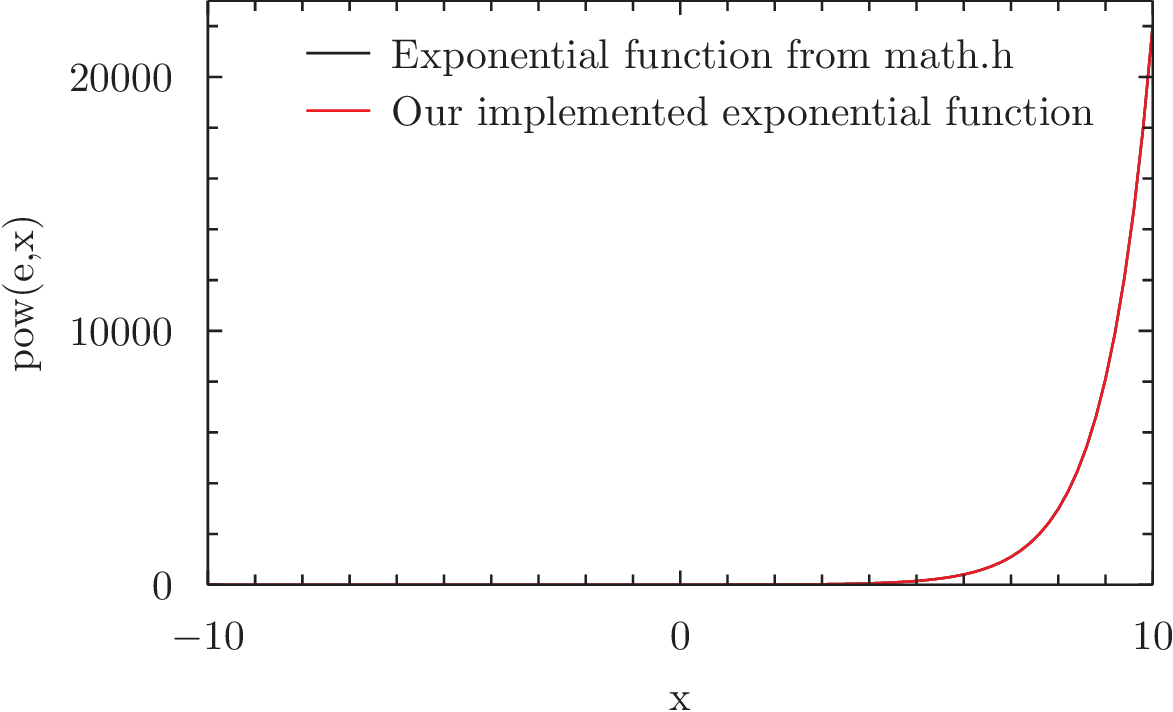
\includegraphics[width=0.8\linewidth]{ex.png}
\caption{Our implementation of the exponential function plotted together with the exponential function given in math.h. As can be seen, our implementation is as precise as the one from math.h}
\label{fig:ex}
\end{figure}
\end{document}
